% Self-contained manuscript patch fragment for the Ritz-certification revision.
% This repository snapshot does not contain a primary manuscript root; integrate
% this fragment into the source root used by the paper build.
% Auto-generated from Ritz certification result files. Do not edit numerical values by hand.
\newcommand{\RitzMacroEta}{4.16e-09}
\newcommand{\RitzMacroEtaBoundary}{lower}
\newcommand{\RitzMacroValidationCriterion}{blocked predictive Gaussian quasi-negative-log-likelihood on held-out full 125-dimensional influence vectors}
\newcommand{\RitzMacroEffectiveNMedian}{375.000}
\newcommand{\RitzMacroP}{125}
\newcommand{\RitzHurricaneFiscalPostDimension}{28}
\newcommand{\RitzHurricaneFiscalPostTraceShare}{0.731}
\newcommand{\RitzHurricaneTopRegion}{New England}
\newcommand{\RitzHurricaneTopYear}{1986}
\newcommand{\RitzHurricaneTopTau}{4.971}
\newcommand{\RitzMaxIdentityError}{8.88e-16}
\newcommand{\RitzMaxCertificateViolation}{0.000}
\newcommand{\RitzMaxGeneralizedEigenpairResidual}{3.22e-13}
\newcommand{\RitzMainLalondeRetainedMass}{0.999}
\newcommand{\RitzMainLalondeP95ExactError}{0.007}
\newcommand{\RitzMainLalondeMaxExactError}{0.011}
\newcommand{\RitzMainLalondeMaxBound}{0.805}
\newcommand{\RitzMainHurricaneR5RetainedMass}{0.661}
\newcommand{\RitzMainHurricaneR5P95ExactError}{0.178}
\newcommand{\RitzMainHurricaneR5MaxExactError}{0.214}
\newcommand{\RitzMainHurricaneR5MaxBound}{1.000 (vacuous)}
\newcommand{\RitzMainHurricaneR15RetainedMass}{0.869}
\newcommand{\RitzMainHurricaneR15P95ExactError}{0.056}
\newcommand{\RitzMainHurricaneR15MaxExactError}{0.065}
\newcommand{\RitzMainHurricaneR15MaxBound}{1.000 (vacuous)}


\subsection{Bounded Stress Diagnostics}
\label{sec:bounded-stress-diagnostics}

Let $\widehat D=\widehat C+\rho I$ and
$\widehat A_\rho(s)=\widehat D^{-1/2}\widehat K(s)\widehat D^{-1/2}$.
For a positive trace-one probe $Q$ and $\lambda>0$, define
$f_\lambda(a)=a/(\lambda+a)$ and
\[
  \widehat q_{\lambda,Q}(s)
  =
  \operatorname{tr}\{Q f_\lambda(\widehat A_\rho(s))\}.
\]
This bounded stress diagnostic is the population object for display. A
finite-rank display is a numerical and interpretive approximation to the same
ridge-relative operator, not a distinct population construction.

Let $P$ be an orthogonal projection and
$\widehat q^P_{\lambda,Q}(s)=
\operatorname{tr}\{Q P f_\lambda(P\widehat A_\rho(s)P)P\}$. Then
\begin{equation}
\boxed{
\left|
\widehat q_{\lambda,Q}(s)-\widehat q^P_{\lambda,Q}(s)
\right|
\le
\operatorname{tr}\{Q(I-P)\}
+
\frac{\|(I-P)\widehat A_\rho(s)P\|}{\lambda}.
}
\label{eq:ritz-stress-bound}
\end{equation}
The first term is omitted probe mass: it is small only when the displayed
subspace contains the directions to which $Q$ assigns mass. The second term is
the Ritz subspace residual: it vanishes when the selected subspace is invariant
for the local ridge-relative operator. Both terms depend on $Q$ and $\lambda$,
so explained unconditional covariance is not by itself a stress certificate.
The proof appears in Appendix~\ref{app:ritz-bound-proof}.

At the dimensions considered here, we use generalized Hermitian interval
extraction through \texttt{scipy.linalg.eigh(..., subset\_by\_value=...)} and
verify selected counts against the exact dense generalized spectrum. FEAST,
rational Krylov, and shift-and-invert methods target the same spectral
projectors in larger problems; no FEAST computation is used in the empirical
results reported here.

\paragraph{Empirical Ritz results.}
Table~\ref{tab:ritz-certification-main} reports exact finite-rank approximation
errors and generic Ritz upper bounds. The generic bound is conservative because
it controls worst-case cross-subspace coupling; a capped value of one is valid
but empirically vacuous. In the generated results, the LaLonde ATE rank-five
error is \RitzMainLalondeMaxExactError, while the corresponding generic bound is
\RitzMainLalondeMaxBound. The hurricane rank-five error is materially larger
(\RitzMainHurricaneR5MaxExactError), supporting the use of rank-five output as
an interpretive display rather than a stand-alone certification. Rank-five
adequacy is probe-specific: a small ATE-probe error does not establish adequacy
for every LaLonde probe.

\begin{table}[!htbp]
\centering
\caption{Finite-rank approximation errors and Ritz bounds}
\label{tab:ritz-certification-main}
\resizebox{\linewidth}{!}{%
\begin{tabular}{@{}llrrrrrr@{}}
\toprule
Application & Probe & $p$ & $R$ & Retained mass & p95 $e_R$ & $\max e_R$ & $\max B_R$ \\
\midrule
LaLonde ATE & overall ATE direction & 11 & 5 & 0.999 & 0.007 & 0.011 & 0.805 \\
Hurricane full fiscal/post probe & fiscal/post block probe & 72 & 5 & 0.661 & 0.178 & 0.214 & 1.000 (vacuous) \\
Hurricane full fiscal/post probe & fiscal/post block probe & 72 & 15 & 0.869 & 0.056 & 0.065 & 1.000 (vacuous) \\
\bottomrule
\end{tabular}
}
\begin{minipage}{0.96\linewidth}
\footnotesize Notes: $e_R$ is the exact full-coordinate stress approximation error at $\lambda_0=1$ and $B_R$ is the capped deterministic Ritz bound. The macro row uses the full-space temporal-resolvent benchmark built from 125-dimensional pre-PCA influence contributions; it is not a full-dimensional latent state-space estimate. Bounds are conditional on the estimated regularized covariance operators.
\end{minipage}
\end{table}


The hurricane principal figure uses the true
\RitzHurricaneFiscalPostDimension-coordinate fiscal/post surface. The highest
amplification cell is \RitzHurricaneTopRegion{} in \RitzHurricaneTopYear{}
with $\tau=\RitzHurricaneTopTau$. Severe-direction counts distinguish
concentrated fragility from multidimensional fragility. Severe-subspace capture
measures whether covariance-PCA contains those directions; low capture means
the largest ridge-relative amplification directions lie outside the dominant
unconditional covariance modes.

\begin{table}[!htbp]
\centering
\caption{Hurricane Ritz certification and severe-direction geometry}
\label{tab:hurricane-ritz-certification}
\scriptsize
\textbf{Panel A. Accuracy}\\[0.3em]
\resizebox{\linewidth}{!}{%
\begin{tabular}{@{}llrrrrrr@{}}
\toprule
Surface and rank & Probe & Trace share & Retained mass & p95 $e_R$ & $\max e_R$ & Share $e_R>.05$ & p95 Ritz subspace residual term \\
\midrule
72-coordinate full event-study surface, R=5 & fiscal/post block probe & 0.603 & 0.661 & 0.178 & 0.214 & 0.718 & 2.716 \\
72-coordinate full event-study surface, R=10 & fiscal/post block probe & 0.723 & 0.759 & 0.135 & 0.144 & 0.574 & 4.298 \\
72-coordinate full event-study surface, R=15 & fiscal/post block probe & 0.807 & 0.869 & 0.056 & 0.065 & 0.133 & 3.971 \\
28-coordinate fiscal/post event-study surface, R=5 & whole-surface soft probe & 0.731 & 0.190 & 0.489 & 0.502 & 1.000 & 1.953 \\
28-coordinate fiscal/post event-study surface, R=10 & whole-surface soft probe & 0.902 & 0.379 & 0.366 & 0.373 & 1.000 & 3.490 \\
28-coordinate fiscal/post event-study surface, R=15 & whole-surface soft probe & 0.964 & 0.567 & 0.259 & 0.294 & 0.877 & 2.564 \\
\bottomrule
\end{tabular}
}
\\[0.8em]
\textbf{Panel B. Severe Geometry}\\[0.3em]
\resizebox{\linewidth}{!}{%
\begin{tabular}{@{}lrrrrrr@{}}
\toprule
Surface and threshold & Median $d$ & Max $d$ & Share $d>0$ & Median $\kappa$ & p90 $\kappa$ & Max generalized-eigenpair residual \\
\midrule
72-coordinate full event-study surface, $a_\star=2$ & 10.000 & 23 & 0.959 & 0.013 & 0.144 & 3.2e-13 \\
72-coordinate full event-study surface, $a_\star=4$ & 3.000 & 12 & 0.836 & 0.006 & 0.301 & 3.2e-13 \\
28-coordinate fiscal/post event-study surface, $a_\star=2$ & 2.000 & 15 & 0.621 & 0.108 & 0.337 & 1.4e-13 \\
28-coordinate fiscal/post event-study surface, $a_\star=4$ & 0.000 & 7 & 0.441 & 0.226 & 0.685 & 1.4e-13 \\
\bottomrule
\end{tabular}
}
\begin{minipage}{0.96\linewidth}
\footnotesize Notes: The restricted surface is the true fiscal/post intersection derived from checked-in surface metadata. Panel A's residual term is $r_R(s)/\lambda$ with $\lambda=1$, where $r_R(s)$ is the Ritz subspace residual. Panel B defines $\kappa_5(s;a_\star)=\|V_5'U_\star(s)\|_F^2/d_\star(s;a_\star)$ when $d_\star>0$. Interval eigenpairs are extracted with \texttt{scipy.linalg.eigh(..., subset\_by\_value=...)} and verified against full dense eigenvalue counts; the reported residual is the numerical generalized-eigenpair residual.
\end{minipage}
\end{table}


The macro appendix is a full-space temporal-resolvent benchmark with
$p=\RitzMacroP$, not a full-dimensional latent state-space fit. Eta is selected
by \RitzMacroValidationCriterion; the selected value is \RitzMacroEta{} and is
classified as \RitzMacroEtaBoundary{} on the generated grid.

\begin{figure}[!htbp]
\centering
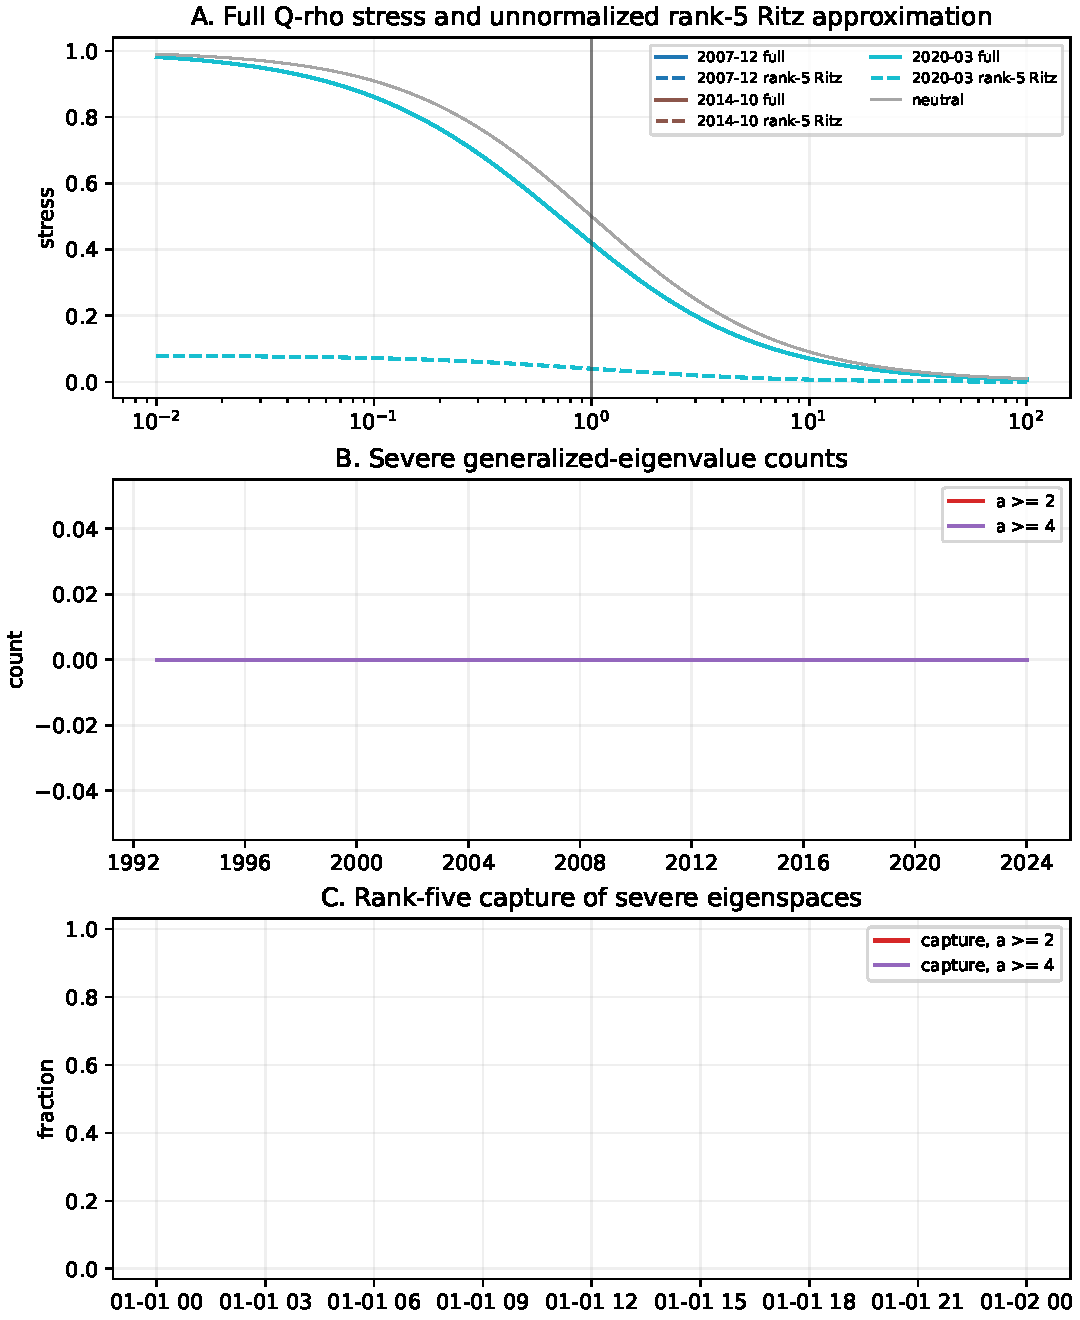
\includegraphics[width=0.96\linewidth]{results/ritz_certification/figures/macro_ritz_interval_spectrum.pdf}
\caption{Macro Ritz stress and interval-spectrum diagnostics. The full calculation is a 125-dimensional temporal-resolvent benchmark. The rank-five curve is the rank-five Ritz approximation to the same full soft-probe stress. Amplification thresholds are ridge-adjusted relative to $\widehat C+\rho I$. The interval-spectrum backend is generalized Hermitian interval extraction; the maximum generalized-eigenpair residual is \RitzMaxGeneralizedEigenpairResidual.}
\label{fig:macro-ritz-interval-spectrum}
\end{figure}

\begin{figure}[!htbp]
\centering
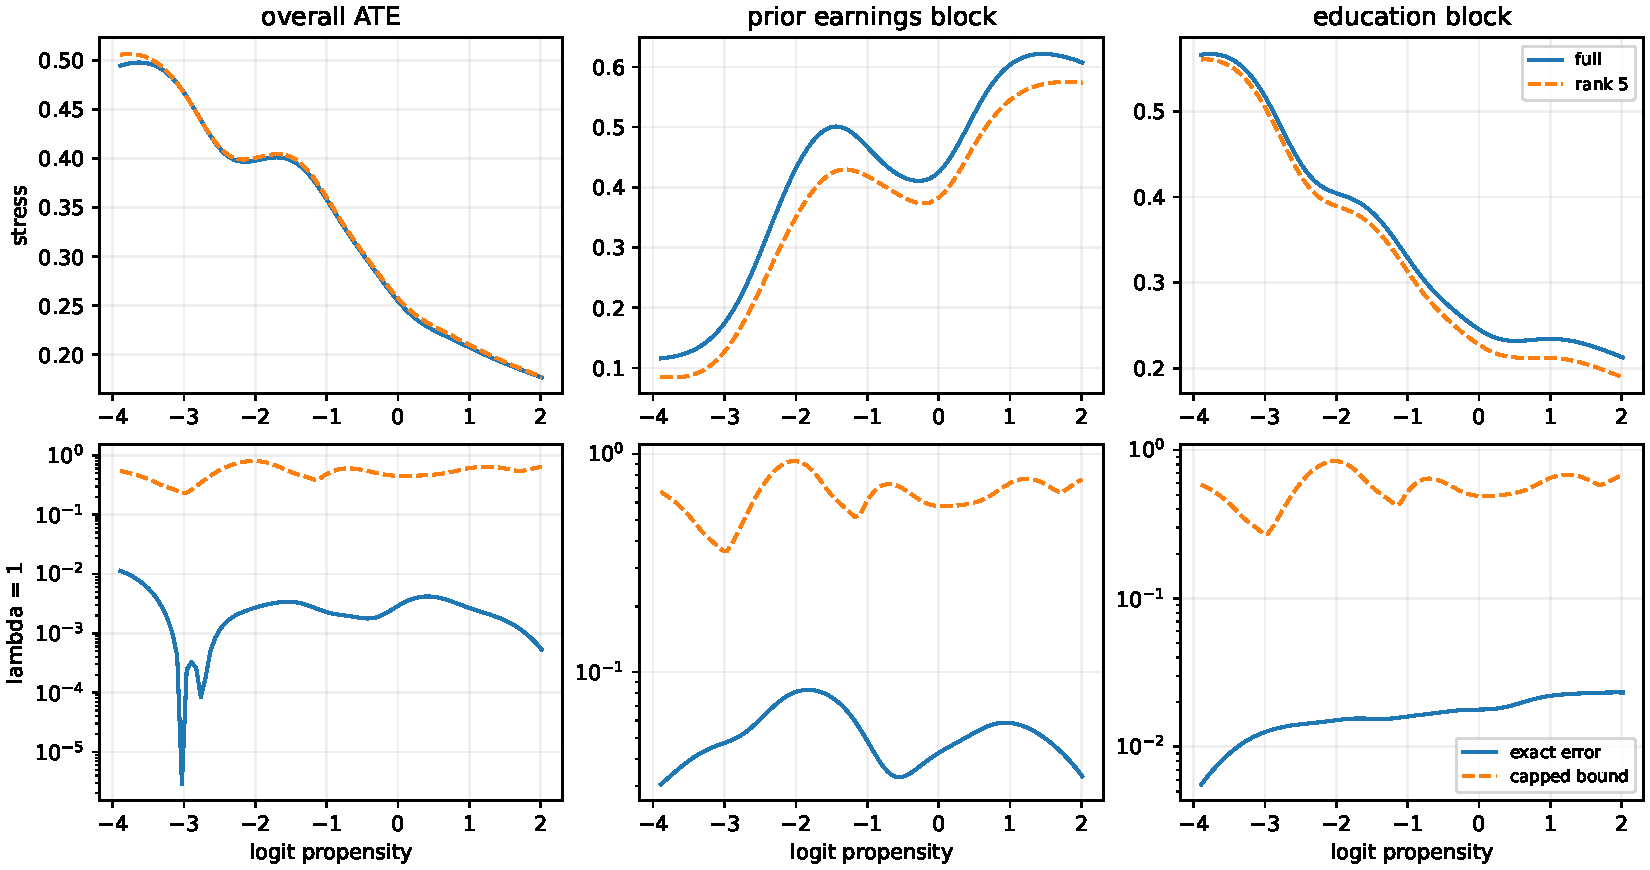
\includegraphics[width=0.96\linewidth]{results/ritz_certification/figures/lalonde_ritz_validation.pdf}
\caption{LaLonde Ritz-bound validation. The low-dimensional application permits exact calculation of full-versus-rank-five error for the overall ATE, prior-earnings, and education probes. The generic bound is verified and conservative because it controls worst-case cross-subspace coupling. All quantities are deterministic conditional on the estimated covariance operators.}
\label{fig:lalonde-ritz-validation}
\end{figure}

\section{Spectral Compression for Interpretation}
\label{app:spectral-compression-interpretation}

Let $\widehat C=V\Lambda V'$ with eigenvalues in descending order and
$V_R=V[:,1\!:\!R]$. The finite-rank Ritz matrix is
\[
  \Theta_R(s)=V_R'\widehat A_\rho(s)V_R
  =
  (\Lambda_R+\rho I)^{-1/2}
  V_R'\widehat K(s)V_R
  (\Lambda_R+\rho I)^{-1/2}.
\]
The empirical code asserts this identity numerically. The approximation
$\operatorname{tr}\{(V_R' Q V_R) f_\lambda(\Theta_R(s))\}$ is therefore a
Galerkin/Ritz display of the same ridge-relative stress operator.

\subsection{Ritz residual certification}
\label{app:ritz-residual-certification}

For $P_R=V_RV_R'$, the Ritz subspace residual is
$\operatorname{Residual}_R(s)=\widehat A_\rho(s)V_R-V_R\Theta_R(s)$ and
$r_R(s)=\|\operatorname{Residual}_R(s)\|_2$. The generic bound used in the
tables is
\[
  B_R(s;\lambda,Q)
  =
  \min\left\{1,\,
  1-\operatorname{tr}(V_R'QV_R)+r_R(s)/\lambda
  \right\}.
\]
The empirical validation metadata reports maximum Ritz identity error
\RitzMaxIdentityError{} and maximum certificate violation
\RitzMaxCertificateViolation.

\subsection{Proof of the Ritz stress bound}
\label{app:ritz-bound-proof}

Let $A=\widehat A_\rho(s)$ and decompose the space as
$P\mathcal H\oplus(I-P)\mathcal H$. Let
$A_0=PAP+(I-P)A(I-P)$ be the block-diagonal part of $A$. Since
$f_\lambda(x)=x(\lambda+x)^{-1}=I-\lambda(\lambda I+x)^{-1}$ is a positive
contraction on positive semidefinite operators,
$0\le f_\lambda((I-P)A(I-P))\le I-P$. Thus, without assuming that $Q$ commutes
with $P$,
\[
\left|
\operatorname{tr}\{Q f_\lambda(A_0)\}
-
\operatorname{tr}\{Q P f_\lambda(PAP)P\}
\right|
\le
\operatorname{tr}\{Q(I-P)\}.
\]
For the remaining term, the resolvent identity gives
\[
f_\lambda(A)-f_\lambda(A_0)
=
\lambda(\lambda I+A)^{-1}(A-A_0)(\lambda I+A_0)^{-1}.
\]
Both resolvents have norm at most $1/\lambda$, and
$A-A_0=(I-P)AP+PA(I-P)$ has norm $\|(I-P)AP\|$. Hence
\[
\|f_\lambda(A)-f_\lambda(A_0)\|
\le
\|(I-P)AP\|/\lambda.
\]
Because $Q$ is positive with trace one,
$|\operatorname{tr}\{Q[f_\lambda(A)-f_\lambda(A_0)]\}|
\le \|f_\lambda(A)-f_\lambda(A_0)\|$. Combining the two inequalities proves
Equation~\eqref{eq:ritz-stress-bound}.
